%\documentclass[12pt]{report}
%\usepackage[margin=2.5cm]{geometry}    % formatting 

\documentclass[english, 12pt, a4paper, online]{article} 
\usepackage{a4wide}

\usepackage{fancyhdr}                  % headers and footers
\usepackage{graphicx, placeins, subfig, float, floatflt, wrapfig}         % Required for inserting images
\usepackage{amsmath,amsfonts,amsfonts} % math
\usepackage{siunitx}                   % typing values with units
\usepackage{biblatex}
\usepackage{tabto}                     % tabs on title page
\usepackage[colorlinks=true, allcolors=blue]{hyperref}  %blue links for titlepage :3
\usepackage{parskip} % paragraph changing
\usepackage[printonlyused, smaller]{acronym}

\usepackage{lipsum} % sample text
\usepackage{listings} % Including code into file
\usepackage{color}

\usepackage{enumitem}       % alphabetical lists

% MAPLE
%Packages for maple
\usepackage{amssymb}
\usepackage{graphicx}
\usepackage{listings}
\usepackage{mathtools}
\usepackage{maple}
\usepackage[utf8]{inputenc}
\usepackage{breqn}
\usepackage{textcomp}

\definecolor{mygreen}{rgb}{0,0.6,0}
\definecolor{mygray}{rgb}{0.5,0.5,0.5}
\definecolor{mymauve}{rgb}{0.58,0,0.82}

\lstset{ %
  backgroundcolor=\color{white},   % choose the background color
  basicstyle=\footnotesize,        % size of fonts used for the code
  breaklines=true,                 % automatic line breaking only at whitespace
  captionpos=b,                    % sets the caption-position to bottom
  commentstyle=\color{mygreen},    % comment style
  escapeinside={\%*}{*)},          % if you want to add LaTeX within your code
  keywordstyle=\color{blue},       % keyword style
  stringstyle=\color{mymauve},     % string literal style
}

\usepackage[toc,page]{appendix} % For appendices



% =========== Setup for page numbering ===========
\pagestyle{fancy}
\renewcommand{\headrulewidth}{0pt}
\fancyhead{}
\fancyfoot{} 
\fancyfoot[R]{\thepage}

\addbibresource{references.bib}

\setlength{\parindent}{0pt}

\begin{document}


% =========== Document chapters ===========
\pagenumbering{roman}
\begin{titlepage}
    \begin{center}
    
        \vspace*{1cm}
        \Huge
        \textbf{SATELLITE AOCS – HOMEWORK \#2}
            
        \vspace{0.5cm}
        \LARGE
        M2TSI - M11 Orbital Mechanics II


            
        \vspace{2cm}
        \Large
        \begin{flushleft}
            \text{Benjamin AKERLUND}  \tab\url{benker-3@student.ltu.se}
            
            
        \end{flushleft}
            
        \vfill
            
        %\includegraphics[width=0.4\textwidth]{Graphics/LTU_logo.png}
        
\includegraphics[width=0.6\linewidth]{Graphics/Vignette logo.png}
        \vfill
   
        
        \begin{flushleft}
            \large
            M2 - Space Technology and Instrumentation (TSI) \\
            Faculty of Science and Engineering (\textit{Faculté sciences et ingénierie}) \\
            Université Toulouse III - Paul Sabatier (UPS)
            %\acl{UPS} \\
            \today
        \end{flushleft}
                   
            
    \end{center}
\end{titlepage}
\addcontentsline{toc}{section}{Preface}
\section*{Preface}

This report is a submission for the \textit{M2TSI - M11 Orbital Mechanics II} course at UPS during the autumn semester of 2024.
%\ac{UPS} during the autumn semester of 2024.
The submission is for the \textit{SATELLITE AOCS – HOMEWORK \#2} assignment as part of the graded assignments for this course.

\textcolor{red}{TODO: something about source code etc?}




%\addcontentsline{toc}{section}{Abstract}
\section*{Abstract}



\begin{table}[h]
    \begin{tabular}{|p{\linewidth}|}
        \hline \\
        Using \ac{SPENVIS}, this report investigates the spacecraft environment for a specific pre-determined orbit corresponding to a so-called Molniya orbit.
        This report analyses the expected spacecraft environment and gives recommendations on design choices: specifically the thickness of solar panel cover glass, the thickness of aluminium shielding for memory devices and the selection of one Integrated Circuit chip over another. 
        \\~\\
        \textit{"\acs{SPENVIS} is \ac{ESA}'s \acf{SPENVIS}, a WWW interface to models of the space environment and its effects; including galactic cosmic rays, solar energetic particles, natural radiation belts, plasmas, gases, meteoroids and debris."} \cite{spenvis_webpage}.
        \\
        \hline
    \end{tabular}
    \label{abbreviations}
\end{table}
\textbf{Keywords:} SPENVIS, ESA, Spacecraft Environment, Space Environment, Single Event Effect, Single Event Upset, CMOS, Solar degradation, 

\vspace{2cm}
        \begin{figure}[h]
            \centering
            \includegraphics[width=0.3\textwidth]{Graphics/spenvislogo.png}
            \hspace{1cm}\includegraphics[width=0.3\textwidth]{Graphics/esa.png}
        \end{figure}
%%% Created: Vincent Brückner
%% define acronym, eg. LTU:              \acro{LTU}{Luleå University of Technology}
%% use in text:                 \ac{LTU} -> first time: Luleå University of Technology (LTU) ;-> all following times: LTU
%% (Note capital letters)
%% force long version in text:  \acf{LTU} -> Luleå University of Technology (LTU)
%% force short version in text: \acs{LTU} -> LTU
%% long version without LTU:    \acl{LTU} -> Luleå University of Technology
%% More info: https://ftp.acc.umu.se/mirror/CTAN/macros/latex/contrib/acronym/acronym.pdf

%% Before publishing: Copy all acronyms into Excel and sort by alphabetic order


\addcontentsline{toc}{section}{Symbols and Abbreviations}
\section*{Symbols and Abbreviations}

\subsection*{Symbols}
\label{subsec:symbols}
List of symbols I guess


%\vfill

\subsection*{Abbreviations}
\label{subsec:abbreviations}

\begin{acronym}[CCSDS] % [longest acronym]
    \acro{PSF}{Point Spread Function}
    \acro{UPS}{Université Toulouse III - Paul Sabatier}
    \acro{LTU}{Luleå University of Technology}
    \acro{ML}{Maximum Likelihood estimator}
\end{acronym}
\tableofcontents
\addcontentsline{toc}{section}{Contents}
\include{} % DO NOT REMOVE

% content chapters
\pagenumbering{arabic}
\section{Local orbital frame}
\label{sec:local}

\begin{itemize}
    \item[-] \textbf{Give the definition of a geocentric inertial reference frame}

    \textit{Geocentric} refers to the centre of the reference frame being the centre of the Earth. 
    Reference frames can typically be divided into \textit{inertial} and \textit{non-inertial} reference frames, where \textit{inertial} means that the frame is not accelerating (or rotating) and is fixed. 
    The orientation of the coordinate axes is fixed relative to distant stars, typically defined by the vernal equinox and the celestial equator.
    Such frames are more often used due to simplification of the calculation of motion laws.
    
    An example of an often-used geocentric inertial reference frame is the Earth-Centric Inertial (ECI).
    
    \item[-] \textbf{Give the definition of the local orbital frame $R_{LOF}$}
    
    A local orbit reference frame Z-, Y- and X-axis are defined as follows:
    \begin{itemize}
        \item $Z_{ol}$ or \textbf{R}: points directly from the centre of the central body (in this case Earth) towards the orbiting object (in this case the satellite), Zenith direction.
        
        \item $Y_{ol}$ or \textbf{W}: points in the direction of the normal positive to the orbital plane.
    
        \item $X_{ol}$ or \textbf{S}: completes the orthonormal trihedron and in this case points in the direction of the satellite's movement along its orbit.
    \end{itemize} 
    
    \begin{figure}[h]
        \centering
        \subfloat[From lecture slides, (R,S,W) vectors (1-2-3)]
        {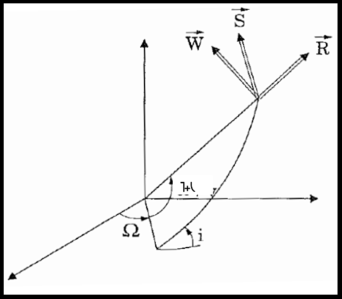
\includegraphics[width=0.4\textwidth]{Graphics/cloe_LOF.png}
        \label{fig:f2-1}}
        %\hfill
        \subfloat[qsw local orbital reference frame]
        {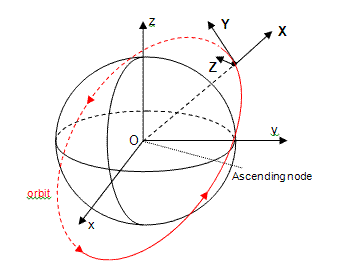
\includegraphics[width=0.45\textwidth]{Graphics/qsw_frame.png}
        \label{fig:f2-2}}
        \caption{The LOF axis can be defined in different ways, such as in (b), where it is the X-axis that follows the radial or zenith direction \cite{ISAE_frames}}
    \end{figure}
    
    
    \newpage
    \item[-] \textbf{Compute the Cubesat local orbital frame vector directions in your geocentric reference frame RE (theoretical computation)}
    
    text


    
    \item[-] \textbf{Make a plot of the local orbital frame vector directions (as a function of time)}

    plot...

    refer to python code in appendix?

    

\end{itemize}
\section{Visibility of a sub satellite point} 

 
\textbf{Let’s consider the point P on Earth located at P (0° latitude, 0°, longitude). }
\begin{itemize}
    \item[-] \textbf{Describe (in plain language) the conditions for the point P to be visible from the CubeSat.}
    \item[-] \textbf{Describe an algorithm that allows to determine if the point P is visible from the CubeSat.}
    \item[-] \textbf{Code this algorithm and show, on a ground map, the points of the orbit which are visible from this point P.}
    \item[-] \textbf{What is the duration of the visibility for a satellite passing at the zenith of P?}
\end{itemize}

 
\vspace{0.5cm}
\begin{itemize}
    \item[-] \textbf{Express the vector (CubeSat, P) in satellite local orbital frame.}
    \item[-] \textbf{Describe an algorithm to compute the direction of the point P in local orbital reference frame.}
    \item[-] Code this algorithm and show, on a 3D plot, the vector wrt time over one orbit.
\end{itemize}
\section{Validation of results}
\label{sec:validation}

\begin{itemize}
    \item[-] \textbf{Use publicly available tools to draw the ISS ground-track at the same epoch and compare it with your results.}
\end{itemize}

Using the ISSTracker tool we can plot a groundtrack of the ISS for the same timeperiod as in Section \ref{sec:ground_track}. 
For this, we first extract the epoch from the telemetry data and arrive at: $2024-10-07 \quad 12:48:15 \quad UTC$.
We can now input this to the ISSTracker (exchanging UTC for $+0000$) and see the correct plot in Figure Section \ref{fig:ISS_validation} below.

From the figure, especially the starting and ending points of the groundtrack, we see that our computed groundtrack matches this fairly well.
Additionally, the orbital period which arrived at in \ref{sec:TLE} of $5576.436740221023 \, s$ or $92.94061233701704 \, min$ matches the orbital period value found online of about $92,9 \, min$ \cite{ISS_tracking_orbitalperiod}.

As such, we can conclude that our method for computing and plotting the groundtrack in Section \ref{sec:TLE} is sound.

\begin{figure}[H]
    \centering
    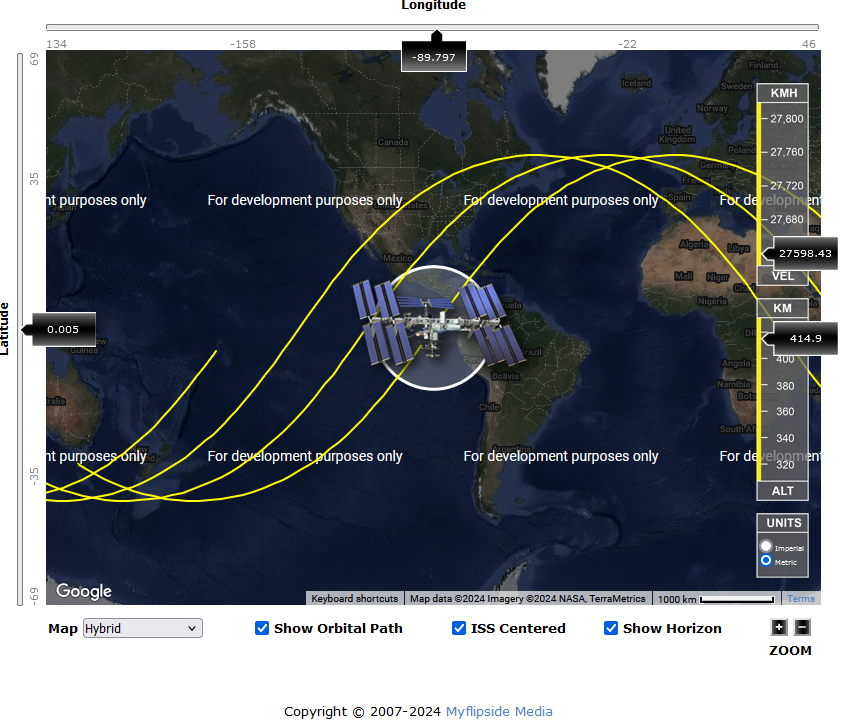
\includegraphics[width=0.8\linewidth]{Graphics/ISS_validation.png}
    \caption{Groundtrack of the ISS drawn at our epoch 2024-10-07 12:48:15+0000 (UTC) using online tool. \cite{ISStracker}}
    \label{fig:ISS_validation}
\end{figure}



\section{Impact of the J2 parameters}
\label{sec:J2}

% ~~~~~~~~~~~~~~~~~~~~~~~~~~~~~~~~
% J2 parameter and it's impact
% ~~~~~~~~~~~~~~~~~~~~~~~~~~~~~~~~
\begin{itemize}
    \item[-] \textbf{What is the $J_2$ parameter and what is its impact on orbit propagation?}
\end{itemize}

The $J_2$ parameter is a dimensionless parameter that quantifies the major effects of the oblateness of Earth on orbits.
With the help of this parameter, we can make more precise predictions of satellite orbits since the Earth is not a perfect spheroid and as such Earth's gravitational field is not that of a perfect spheroid. 
The oblateness of Earth causes a variation of the gravitational field also with latitude, i.e., the angular distance from the equator (or pole), as compared to the only variation being caused by the radial distance from the centre of the spheroid model of the planet. \cite{coursebook_ch4}

$J_2$ is not a universal constant but varies depending on which planetary body is studied. 
A table of $J_2$ parameters for the planets in our solar system can be seen in the coursebook in table 4.3 \cite{coursebook_ch4}, and from here we read for on oblateness of $0.003353$ of Earth: 
\begin{equation}
    J_{2, E} = 1.08263 \times 10^{-3}
\end{equation}

Oblateness causes the right ascension, $\Omega$, and the argument of periapsis, $\omega$, to vary significantly with time. 
This is described mathematically with functions for the rate of change:
\begin{equation}
    \begin{split}
        &\Dot{\Omega} = - \left[ 
            \frac{3} {2} 
            \frac{\sqrt{\mu} J_2 R^2} {(1-e^2)^2 a^{7/2}}
            \right]
            cos \, i\\
        &\Dot{\omega} = - \left[ 
            \frac{3} {2} 
            \frac{\sqrt{\mu} J_2 R^2} {(1-e^2)^2 a^{7/2}}
        \right] 
        \left(
            \frac{5}{2} sin^2 \, i - 2
        \right)
    \end{split}
\end{equation}

This variation, or drift, is such that for:
\begin{itemize}
    \item[] $0 <= i < 90^{\circ}$ then $\Dot{\Omega} < 0$. 
    \item[] $90^{\circ} < i <= 180^{\circ}$ then $\Dot{\Omega} > 0$. 
    \item[] $0 <= i < 63.4^{\circ}$ or $116.6^{\circ} < i <= 180^{\circ}$  then $\Dot{\omega} < 0 \xrightarrow{}$ the perigee advances in the direction of the motion of the satellite.
    \item[] $63.4^{\circ} < i <= 116.6^{\circ}$ then $\Dot{\omega}$ regresses $\xrightarrow{}$ the perigee advances in the opposite direction of the motion of the satellite.
\end{itemize}

\underline{That means for prograde orbits, such as the ISS, the node line drifts westward and the} \\
\underline{perigee advances in the direction of the motion of the ISS.}
The effect of oblateness on the rates of change of $\Omega$ and $\omega$ is greatest at low inclination orbits, i.e., when the orbit is near the equatorial bulge for longer portions of each revolution. 
This effect also decreases as the semi-major axis of an orbit increases, since the satellite is further away from the bulge and its gravitational influence.

It also turns out that the J2 effect produces zero time-averaged variations of the inclination, eccentricity, angular momentum, and semimajor axis. \cite{coursebook_ch4}




% ~~~~~~~~~~~~~~~~~~~~~~~~~~~~~~~~
% Ascending node drift for ten orbits 
% ~~~~~~~~~~~~~~~~~~~~~~~~~~~~~~~~
\begin{itemize}
    \item[-] \textbf{What is the ascending node drift for ten orbits for the ISS due to the $J_2$ parameter?}
\end{itemize}

Calculated in Maple to: 
\[\Dot{\Omega} = -3.195150212^{\circ} \]


% ~~~~~~~~~~~~~~~~~~~~~~~~~~~~~~~~
% J22 parameter 
% ~~~~~~~~~~~~~~~~~~~~~~~~~~~~~~~~
\begin{itemize}
    \item[-] \textbf{What is the $J_{22}$ parameter and when should it be accounted for?}
\end{itemize}

The J22 parameter is a second-order harmonic term that accounts for the effects of the Earth's oblateness even beyond the J2 parameter. 
While J2 represents Earth's equatorial bulge, J22 represents the non-symmetrical gravitational field of the Earth due to different landmasses around the globe and Earth being more "potato"-shaped than an oblate "egg". 
As such, the J22 parameter should be accounted when wanting very precise orbital propagations over very long durations, when this could be visible. 


% ~~~~~~~~~~~~~~~~~~~~~~~~~~~~~~~~
% Orbit propagation without/with J2
% ~~~~~~~~~~~~~~~~~~~~~~~~~~~~~~~~
\begin{itemize}    
    \item[-] \textbf{Write a propagation without J2 and propagate the orbit of the ISS during 10 orbits without J2.}
\end{itemize}

\begin{itemize} 
    \item[-] \textbf{Write a propagation with J2 and propagate the orbit of the ISS during 10 orbits with J2.}
\end{itemize}

The idea for this would be to update the TLE each minute with the new $\Omega$ and $\omega$ values after calculating the rate of change in minutes.
Then plotting each minute with the updated values in blue, would show how the orbit propagates according J2.

A plot of the orbit propagation for 10 orbits without (red) and with $J_2$ (blue) can be seen below in Figure \ref{fig:ISS_plot_J2}.

\begin{figure}[H]
    \centering
    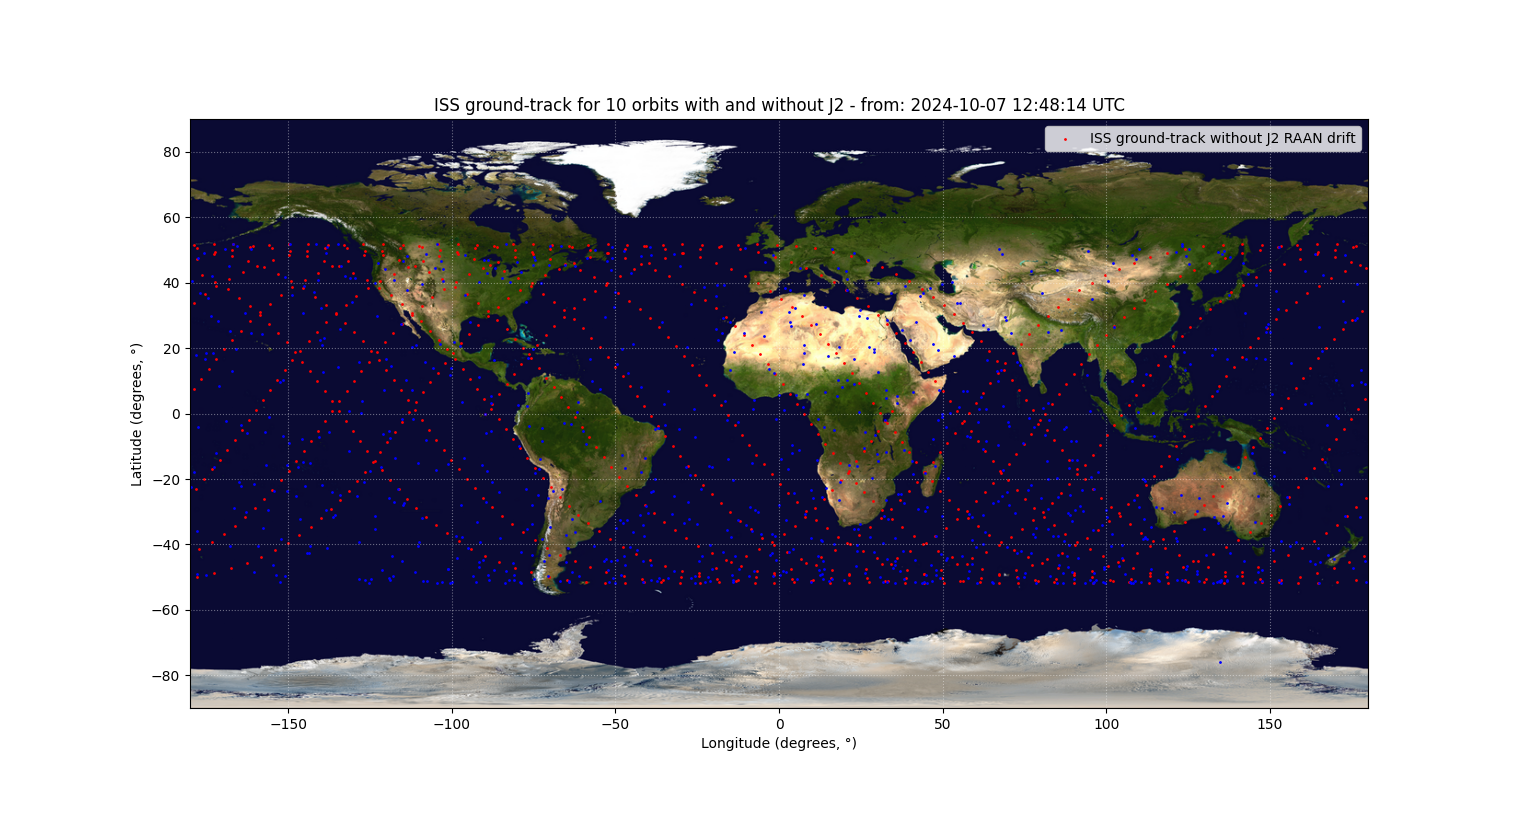
\includegraphics[width=1\linewidth]{Graphics/ISS_plot_J2.png}
    \caption{Plot of computed ISS orbit propagation ground track for 10 orbits without/with J2 using code from Appendix \ref{sec:Appendix_A}.}
    \label{fig:ISS_plot_J2}
\end{figure}
%\section{Interplanetary transfer $\Delta V$ computation}
\label{sec:interplanetary_transfer}

\textbf{Now let’s take a mission which consists of a heliocentric transfer from the vicinity of Earth to the vicinity of Mars. 
The initial mass, M0=20,000, starts just outside Earth’s sphere of influence (SOI) and finishes just outside Mars’ SOI.
}

\textbf{Consider a two-impulse heliocentric Hohmann transfer and calculate the total $\Delta V$ needed for the mission. 
Assume no staging is involved. 
With a jet velocity of c = 4500 m/s and a specific impulse of I = 459 s (typical for a LOX-PLH rocket).}
\begin{itemize}
    \item[-] \textbf{What is the total delta V needed to arrive near Mars?}
\end{itemize}


\textbf{Additionally, assume that 5\% of the initial mass (1 000 kg) consists of the structure and engine, with the remainder allocated for the payload.}
\begin{itemize}
    \item[-] \textbf{What is the mass of this payload?}
    \item[-] \textbf{What is the duration of the transfer?}
    \item[-] \textbf{Plot this transfer} 
\end{itemize}




Got stuck on J2 propagation plotting and ran out of time...


% =========== REFERENCES ===========
\addcontentsline{toc}{section}{References}
\section*{References}
\label{sec:references}
\printbibliography[heading=none]

\begin{appendices}

\section{Python code}
\label{sec:Appendix_A}

\begin{lstlisting}[frame=single, language=Python, numbers=left]
import math
import pytz
from dateutil.relativedelta import relativedelta
from skyfield.api import load, wgs84, EarthSatellite
import matplotlib
matplotlib.use('QtAgg')
import matplotlib.pyplot as plt
from datetime import timedelta

timescale = load.timescale()

# two-line elements given in homework assignment, updated according to email
line1 = '1 25544U 98067A   24281.53350623  .00033313  00000+0  60150-3 0  9991'
line2 = '2 25544  51.6369 118.9253 0008961  46.9406 313.2331 15.49376493475973'
satellite = EarthSatellite(line1, line2, 'ISS (ZARYA)', timescale)


''' 
Part 1: 
Two lines elements (TLE)
* Orbital elements from TLE-data:
    * read keplerian orbital elements from TLE-data
    * calculate semi-major axis from mean motion and orbital time
    * print values
'''
# Orbital elements
eccentricity = line2[26:33]
inclination = line2[8:16]
right_ascension = line2[17:25]
argument = line2[34:42]
mean_anomaly = line2[43:51]
mean_motion = line2[52:63]

# Calculate semi-major axis
T = 24*60*60/float(mean_motion)
mu = 3.986*10**14
a = (((T**2) * mu) / (4 * (math.pi ** 2)))**(1/3)

# Printing values
print("======== Orbital elements ========")
print("eccentricity: ", eccentricity)
print("inclination: ", inclination)
print("right ascension: ", right_ascension)
print("argument of periapsis: ", argument)
print("mean anomaly: ", mean_anomaly)
print("mean motion: ", mean_motion)

print("Orbital period: ", T, "s or", T/60, "min")
print("Semi-major axis: ", a/1000, "km")
print("==================================")



''' Part 2: 
Ground track computation
* get starting time from epoch
* set timescale and calculate subpoints (latitude and longitude)
* Plot the groundtrack onto an existing map 
    * image credits: https://upload.wikimedia.org/wikipedia/commons/2/23/Blue_Marble_2002.png 
'''
# Get current time in a timezone-aware fashion from the epoch
tz = pytz.timezone('UTC')
dt = satellite.epoch.astimezone(tz)
print()
print(satellite)
print(f"Exectution time: {dt:%Y-%m-%d %H:%M:%S %Z}\n")

# if statement added for ease of use...
if input("Do you want to plot for part 2 [y/n]?") == "y":
    # Split 3 orbits (3*92.94061233 minutes) into 400 evenly spaced Timescales as indicated by points
    # 400 chosen for map visibility reasons, could be 101 ==> one plot every 2 min + endpoints
    orbits_min = 3 * T / 60
    t0 = timescale.utc(dt)
    t1 = timescale.utc(dt + relativedelta(minutes=orbits_min))
    timescales = timescale.linspace(t0, t1, 400)

    # calculate the latitude and longitude subpoints.
    geocentrics = satellite.at(timescales)
    subpoints = wgs84.subpoint_of(geocentrics)
    latitude = subpoints.latitude.degrees
    longitude = subpoints.longitude.degrees

    # Load background image
    background_image_path = r'C:\Users\benja\PycharmProjects\groundtrack\earth.jpg'
    background_img = plt.imread(background_image_path)

    # Create the plot
    plt.figure(figsize=(15.2, 8.2))
    plt.imshow(background_img, extent=[-180, 180, -90, 90])

    # Plot the ground track
    title = f"ISS ground-track from: {dt:%Y-%m-%d %H:%M:%S %Z}"
    plt.scatter(longitude, latitude, label="ISS ground-track", color='red', marker='o', s=1)
    plt.xlabel("Longitude (degrees, \N{DEGREE SIGN})")
    plt.ylabel("Latitude (degrees, \N{DEGREE SIGN})")
    plt.title(title)

    # Show the plot
    plt.legend()
    plt.grid(True, color='w', linestyle=":", alpha=0.4)
    plt.show()



''' Part 4: 
Impact of the J2 parameters
* something
* plot scatter points without J2 RAAN drift in red
* plot scatter points with J2 RAAN drift in blue
'''
if input("Do you want to plot for part 4 [y/n]?") == "y":
    # Split 3 orbits (3*92.94061233 minutes) into 1000 evenly spaced Timescales as indicated by points
    # 400 chosen for map visibility reasons, could be 101 ==> one plot every 2 min + endpoints
    orbits_min = int(10 * T / 60)
    t0 = timescale.utc(dt)
    t1 = timescale.utc(dt + relativedelta(minutes=orbits_min))
    timescales = timescale.linspace(t0, t1, orbits_min+1)

    # calculate the subpoints.
    geocentrics = satellite.at(timescales)
    subpoints = wgs84.subpoint_of(geocentrics)

    '''# Print a nicely-formatted, tab-delimited time, latitude, and longitude.
    for t, lat, lon in zip(timescales,
                           subpoints.latitude.degrees,
                           subpoints.longitude.degrees):
        print(f"{t.astimezone(tz):%Y-%m-%d %H:%M:%S}\t{lat:8.2f}\t{lon:8.2f}")
'''

    # Load background image
    background_image_path = r'C:\Users\benja\PycharmProjects\groundtrack\earth.jpg'
    background_img = plt.imread(background_image_path)
    latitude = subpoints.latitude.degrees
    longitude = subpoints.longitude.degrees

    # Create the plot
    plt.figure(figsize=(15.2, 8.2))
    plt.imshow(background_img, extent=[-180, 180, -90, 90])

    # Plot the ground track with and without J2 RAAN drift (red and blue)
    title = f"ISS ground-track for 10 orbits with and without J2 - from: {dt:%Y-%m-%d %H:%M:%S %Z}"
    plt.xlabel("Longitude (degrees, \N{DEGREE SIGN})")
    plt.ylabel("Latitude (degrees, \N{DEGREE SIGN})")
    plt.title(title)

    # plot without J2 drift
    plt.scatter(longitude, latitude, label="ISS ground-track without J2 RAAN drift", color='red', marker='o', s=1)

    # plot with J2 drift (new longitude and latitude vector
    # calculate the subpoints for changing RAAN and argument of perigee
    # both change every second, so for each e.g. minute we can calculate a new
    # also need a new dt for each iteration...
    # Get current time in a timezone-aware fashion from the epoch
    Omega = str(118.9253)
    omega = str(46.9406)
    for a in range(orbits_min):
        # two-line elements given in homework assignment, updated according to email
        #line1 = '1 25544U 98067A   24281.53350623  .00033313  00000+0  60150-3 0  9991'
        #line2 = '2 25544  51.6369 118.9253 0008961  46.9406 313.2331 15.49376493475973'
        line1 = '1 25544U 98067A   24281.53350623  .00033313  00000+0  60150-3 0  9991'
        line2 = '2 25544  51.6369 {:} 0008961  {:} 313.2331 15.49376493475973'.format(Omega, omega)
        satellite = EarthSatellite(line1, line2, 'ISS (ZARYA)', timescale)

        t0_2 = timescale.utc(dt)
        t1_2 = timescale.utc(dt + relativedelta(minutes=1))
        timescales2 = timescale.linspace(t0_2, t1_2, 1)
        geocentrics2 = satellite.at(timescales2)
        subpoints2 = wgs84.subpoint_of(geocentrics2)
        latitude2 = subpoints2.latitude.degrees
        longitude2 = subpoints2.longitude.degrees
        plt.scatter(longitude2, latitude2, color='blue', marker='o', s=1)

        # update variables
        dt = dt + timedelta(0,60)
        Omega = str(float(Omega) - 0.003437840715)
        omega = str(float(omega) + 0.002564598683)



    # Show the plot
    plt.legend()
    plt.grid(True, color='w', linestyle=":", alpha=0.4)
    plt.show()







\end{lstlisting}


\newpage
\section{Maple calculations}
\label{sec:Maple}
\begin{Maple Normal}
\textbf{M11 Orbital Mechanics II - Homework \#1 }
\end{Maple Normal}
\begin{Maple Normal}
1. Two lines Elements (TLE)
\end{Maple Normal}
\begin{Maple Normal}

\end{Maple Normal}
\begin{Maple Normal}
Orbital parameters:
\end{Maple Normal}
\begin{Maple Normal}
{$ \displaystyle \mathit{ecc} \coloneqq  0.0008961\colon  $}
\end{Maple Normal}
\begin{Maple Normal}
{$ \displaystyle i \coloneqq  51.6369\colon  $}
\end{Maple Normal}
\begin{Maple Normal}
{$ \displaystyle i_{\mathit{rad}}\coloneqq \frac{i \cdot \pi}{180}\colon  $}
\end{Maple Normal}
\begin{Maple Normal}
{$ \displaystyle \Omega \coloneqq  118.9253\colon  $}
\end{Maple Normal}
\begin{Maple Normal}
{$ \displaystyle \mathrm{omega}\coloneqq  46.9406\colon  $}
\end{Maple Normal}
\begin{Maple Normal}

{$ \mathrm{nu}\coloneqq  313.2331\colon  $}
\end{Maple Normal}
\begin{Maple Normal}
{$ \displaystyle n \coloneqq  15.49376493\colon  $}
\end{Maple Normal}
\begin{Maple Normal}

\end{Maple Normal}
\begin{Maple Normal}
Constants:
\end{Maple Normal}
\begin{Maple Normal}
{$ \displaystyle \mu\coloneqq  3.986\cdot 10^{14}\colon  $}
\end{Maple Normal}
\begin{Maple Normal}

\end{Maple Normal}
\begin{Maple Normal}
{$ \displaystyle J_{2}\coloneqq  1.08263\cdot 10^{-3}\colon  $}
\end{Maple Normal}
\begin{Maple Normal}
{$ \displaystyle R_{E}\coloneqq 6378\cdot 10^{3}\colon  $}
\end{Maple Normal}
\begin{Maple Normal}
(at the equator)
\end{Maple Normal}
\begin{Maple Normal}

\end{Maple Normal}
\begin{Maple Normal}
Orbital period in seconds and minutes:
\end{Maple Normal}
\begin{Maple Normal}
{$ \displaystyle T_{s}\coloneqq \frac{24\cdot 60\cdot 60}{n} $}
\end{Maple Normal}
% \mapleresult
\begin{dmath}\label{(1)}
T_{s}\coloneqq  5576.436740
\end{dmath}
\begin{Maple Normal}
{$ \displaystyle T_{\min}\coloneqq \frac{T_{s}}{60} $}
\end{Maple Normal}
% \mapleresult
\begin{dmath}\label{(2)}
T_{\min}\coloneqq  92.94061233
\end{dmath}
\begin{Maple Normal}

\end{Maple Normal}
\begin{Maple Normal}
Semi-major axis calculattions [m]: 
\end{Maple Normal}
\mapleinput
{$ \displaystyle a \coloneqq (\frac{T_{s}^{2}\,\cdot \,\mu}{4\cdot \pi^{2}})^{\mathit{(\frac{1}{3})}} $}

% \mapleresult
\begin{dmath}\label{(3)}
a \coloneqq  6.796683381\times 10^{6}
\end{dmath}
\begin{Maple Normal}
{$ \displaystyle a_{\mathit{km}}=a \cdot 10^{-3} $}
\end{Maple Normal}
% \mapleresult
\begin{dmath}\label{(4)}
a_{\mathit{km}}= 6796.683381
\end{dmath}
\begin{Maple Normal}
Rate of change for 
{$ \Omega \colon  $} and 
{$ \omega \colon  $}
\end{Maple Normal}
\begin{Maple Normal}
{$ \displaystyle \Omega_{\mathit{dot}}\coloneqq -(\frac{3}{2}\cdot \frac{\mathrm{sqrt}(\mathrm{mu})\cdot J_{2}\cdot R_{E}^{2}}{(1-\mathit{ecc}^{2})^{2}\cdot a^{\frac{7}{2}}})\cdot \cos (i_{\mathit{rad}})\cdot \frac{180}{\mathrm{Pi}}\cdot 60 $}
\end{Maple Normal}
% \mapleresult
\begin{dmath}\label{(5)}
\Omega_{\mathit{dot}}\coloneqq - 0.003437840715
\end{dmath}
\begin{Maple Normal}
{$ \displaystyle \omega_{\mathit{dot}}\coloneqq -(\frac{3}{2}\cdot \frac{\mathrm{sqrt}(\mathrm{mu})\cdot J_{2}\cdot R_{E}^{2}}{(1-\mathit{ecc}^{2})^{2}\cdot a^{\frac{7}{2}}})\cdot (\frac{5}{2}\cdot \sin(i_{\mathit{rad}})^{2}-2)\cdot \frac{180}{\mathrm{Pi}}\cdot 60 $}
\end{Maple Normal}
% \mapleresult
\begin{dmath}\label{(6)}
\omega_{\mathit{dot}}\coloneqq  0.002564598683
\end{dmath}
\begin{Maple Normal}

\end{Maple Normal}
\begin{Maple Normal}

\end{Maple Normal}
\begin{Maple Normal}
{$ \displaystyle \frac{10\cdot T_{\min}}{3000} $}
\end{Maple Normal}
% \mapleresult
\begin{dmath}\label{(7)}
 0.3098020411
\end{dmath}
\begin{Maple Normal}

\end{Maple Normal}




\end{appendices}

\end{document}
